\documentclass[10pt,a4paper]{article}

\usepackage[utf8]{inputenc}
\usepackage[T1]{fontenc}
\usepackage{lmodern}
\usepackage{graphicx}
\usepackage{color}
\usepackage{xcolor}
\usepackage{geometry}
\usepackage{parskip}
\usepackage[brazil]{babel}
\usepackage[hidelinks]{hyperref}
\usepackage{listings}
\usepackage{placeins}
\usepackage{amsmath}
\usepackage{amssymb}

\geometry{
	a4paper,
	left=2cm,
	right=2cm,
	top=2cm,
	bottom=2cm,
}

\definecolor{dkgreen}{rgb}{0,0.4,0}
\definecolor{dkblue}{rgb}{0,0,0.6}
\definecolor{dkred}{rgb}{0.5,0,0}
\definecolor{ltblue}{rgb}{0.1,0.1,0.9}
\definecolor{gray}{rgb}{0.5,0.5,0.5}
\definecolor{green}{rgb}{0,0.6,0}
\definecolor{orange}{rgb}{0.75,0.25,0}
\colorlet{lessOrange}{orange!70!gray}

\lstset{frame=tb,
	language=C++,
	aboveskip=3mm,
	belowskip=3mm,
	showstringspaces=false,
	columns=flexible,
	basicstyle={\small\ttfamily},
	numbers=none,
	literate={~}{{\raisebox{-0.7ex}{\texttt{\char`~}}}}1,
	numberstyle=\tiny\color{gray},
	keywordstyle=\color{dkblue},
	commentstyle=\color{gray},
	identifierstyle=\color{lessOrange},
	morecomment=[l][\color{dkgreen}]{\#},
	stringstyle=\color{dkgreen},
	breaklines=true,
	breakatwhitespace=true,
	tabsize=4,
	morekeywords={
		uniform, layout, in, out, vec2, vec3, vec4, mat2, mat3, mat4,
		sampler2D, samplerCube, discard, image2D, readonly, ivec2,
		GLuint, GLint, GLchar, GLsizei, GLenum, GLfloat, GLboolean,
		GLvoid, GLbitfield, GLsync, GLuint64, GLintptr, GLsizeiptr,
		atomic_uint, flat, smooth
	}
}

\newcommand{\N}{\mathbb{N}}
\newcommand{\R}{\mathbb{R}}
\newcommand{\C}{\mathbb{C}}
\newcommand{\I}{\mathbb{I}}
\newcommand{\separator}{\noindent\makebox[\textwidth]{\rule{\textwidth}{0.4pt}}}
\newcommand{\vs}{\vspace{0.2cm}}

\title{TP3 - EDN}
\author{Artur Fonseca Costa}
\date{}

\begin{document}

\maketitle



O código completo pode ser encontrado \href{https://github.com/Tuzass/EDN}{aqui}.

\vspace{-0.2cm}
\separator

2.1. A série de senos de $u(x, t)$ é dada por
\[u(x, t) = \sum_{n = 1}^{\infty} b_n e^{- n^2 \pi^2 t} \sin(n \pi x), \text{ onde } b_n = 2 \int_0^1 f(x) \sin(n \pi x) \, dx.\]
Como a função $f(x)$ é definida por partes, tem-se
\begin{flalign}
	b_n &= 2 \left( \int_0^{1/2} 2x \sin(n \pi x) \, dx + \int_{1/2}^1 (2 - 2x) \sin(n \pi x) \right) \nonumber \\
	&= 4 \int_0^{1/2} x \sin(n \pi x) \, dx + 4 \int_{1/2}^1 \sin(n \pi x) \, dx - 4 \int_{1/2}^1 x \sin(n \pi x) \, dx \nonumber \\
	&= 4 \left[ -\frac{x}{n \pi} \cos(n \pi x) + \frac{1}{n^2 \pi^2} \sin(n \pi x) \right]\Bigg\vert_0^{1/2} + 4 \left[ \frac{x - 1}{n \pi} \cos(n \pi x) - \frac{1}{n^2 \pi^2} \sin(n \pi x)\right]\Bigg\vert_{1/2}^1 \nonumber \\
	&= \frac{8}{n^2 \pi^2} \sin\left(\frac{n \pi}{2}\right). \nonumber
\end{flalign}
Nota-se que os coeficientes pares são nulos. Então, a solução é dada por
\[u(x, t) = \frac{8}{\pi^2} \sum_{n = 0}^{\infty} \frac{(-1)^n}{(2k + 1)^2} e^{-(2k + 1)^2 \pi^2 t} \sin((2n + 1) \pi x),\]
e a soma parcial de $k$ termos é
\[u_k(x, t) = \frac{8}{\pi^2} \sum_{n = 0}^{k} \frac{(-1)^n}{(2k + 1)^2} e^{-(2k + 1)^2 \pi^2 t} \sin((2n + 1) \pi x).\]
Sendo $|\sin(x)| \leq 1$ para todo $x \in \R$ e $|e^{-x}| \leq 1$ para todo $x \in [0, \infty)$, pode-se aproximar a solução com
\[|u - u_k| \leq \frac{8}{\pi^2} \sum_{n = k + 1}^{\infty} \frac{1}{(2k + 1)^2} \leq \frac{8}{\pi^2} \int_k^{\infty} \frac{1}{(2x + 1)^2} \, dx = \frac{4}{\pi^2 (2k + 1)}.\]
O erro desejado é $\varepsilon \leq 0.01$, então basta que $|u - u_k| \leq 0.01$:
\[\frac{4}{\pi^2 (2k + 1)} \leq 0.01 \longrightarrow 2k + 1 \geq \frac{4}{0.01 \pi^2} \approx 40.5 \longrightarrow k \geq 20.\]
Logo, basta usar os primeiros 21 termos $\left( \sum_{n = 0}^{20} \right)$ para obter um erro inferior a 0.01.



\vs
2.2. O método das linhas depende de uma escolha de aproximação para $\partial_t u(x, t)$. Foi escolhido o método de Euler, cuja aplicação ao método das linhas é o método das diferenças progressivas:
\[u_{m, j + 1} = u_{m, j} + \mu (u_{m - 1, j} - 2 u_{m, j} + u_{m + 1, j}),\]
onde $mu = \frac{\Delta t}{(\Delta x)^2}$. Sua implementação pode ser vista abaixo:
\clearpage
\begin{lstlisting}
void ftcs(double x_0, double X, double t_0, double T, double dx, double dt){
	const int M = (X - x_0) / dx;
	const int N = (T - t_0) / dt;
	const double mu {dt / (dx * dx)};

	for (int m {}; m <= M; m++)
	x[m] = x_0 + m * dx;

	for (int j {}; j <= N; j++)
	t[j] = t_0 + j * dt;

	for (int m {}; m <= M; m++)
	u[0][m] = f(x_0 + m * dx);

	for (int j {}; j <= N; j++){
		u[j][0] = 0;
		u[j][M] = 0;
	}

	for (int j {}; j < N; j++)
	for (int m {1}; m <= M - 1; m++)
	u[j + 1][m] = u[j][m] + mu * (u[j][m - 1] - 2 * u[j][m] + u[j][m + 1]);
}
\end{lstlisting}

Sabe-se que esse método é convergente se $\mu \leq \frac{1}{2}$, então os testes foram feitos com essa restrição em mente. Em casos onde essa restrição foi ignorada ($\Delta t = 0.0001$ e $\Delta x = 0.01$, por exemplo), o programa produziu valores inválidos (\texttt{NaN}) e não foi possível gerar o mapa de calor. Foram testados os valores $\Delta x = 0.01, 0.02, 0.05$:

\begin{figure}[ht!]
	\centering
	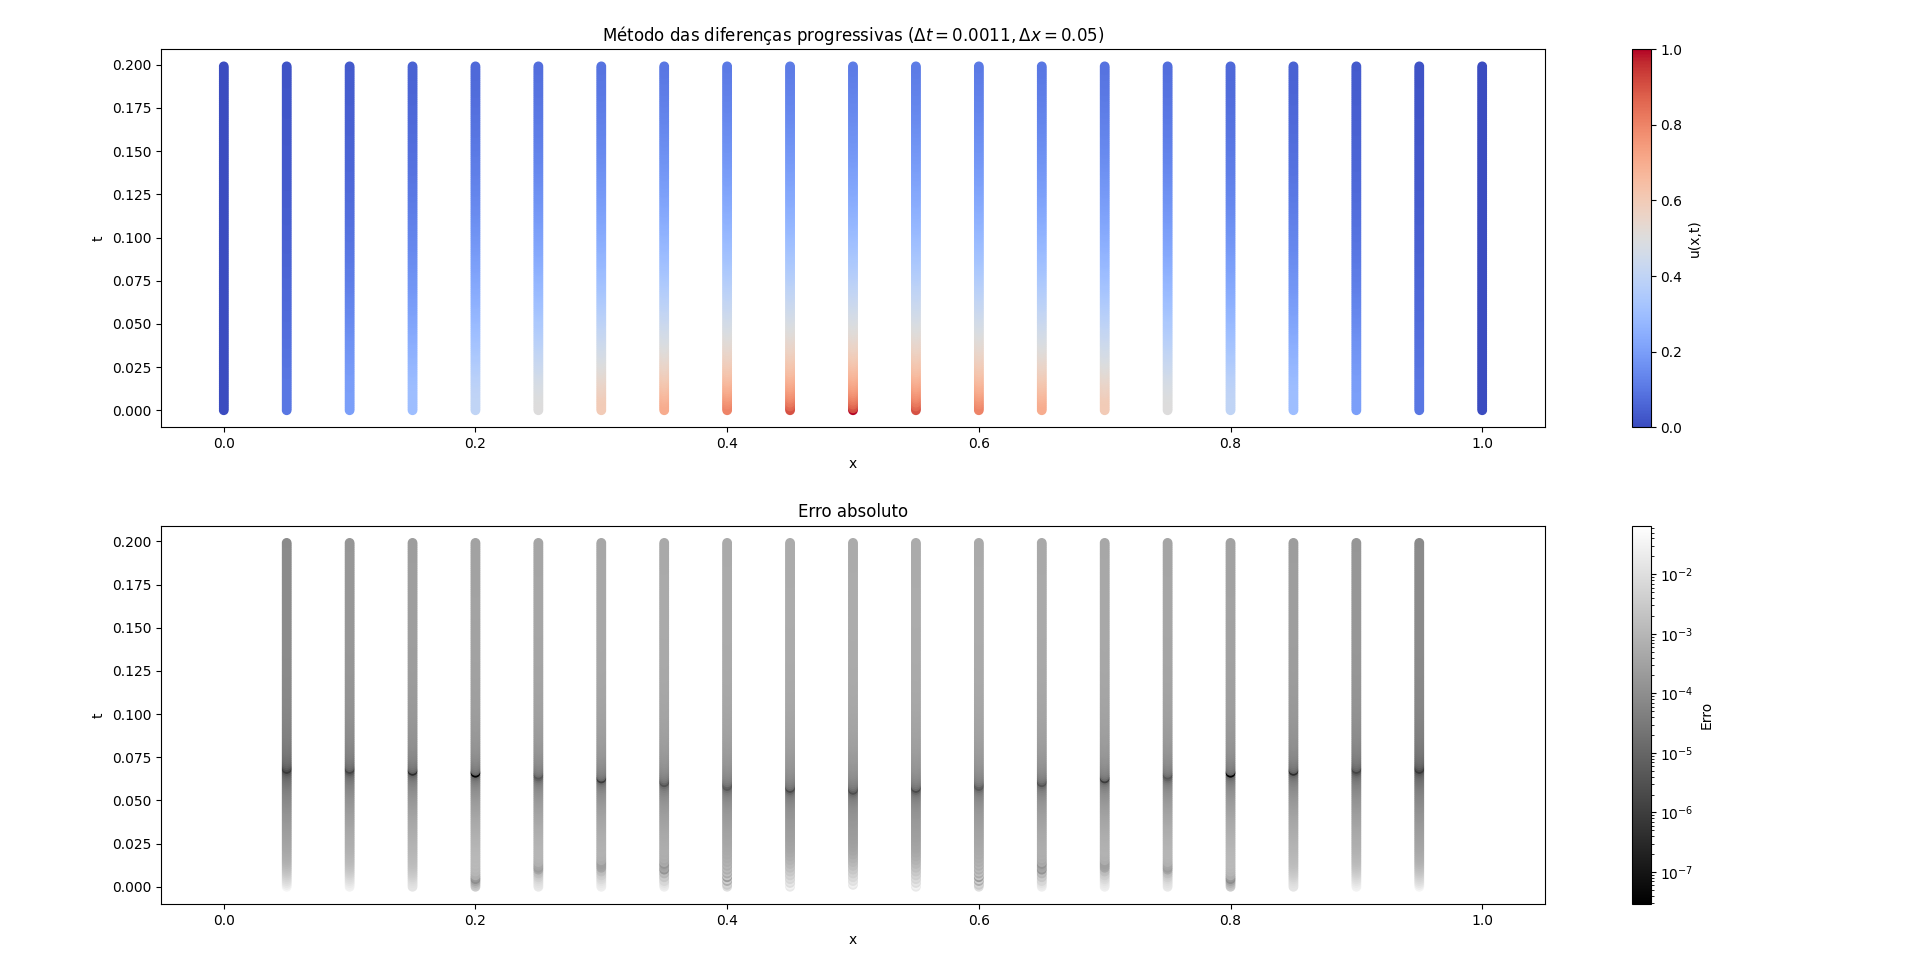
\includegraphics[width=0.7\textwidth]{img/ftcs_005.png}
\end{figure}

\begin{figure}[ht!]
	\centering
	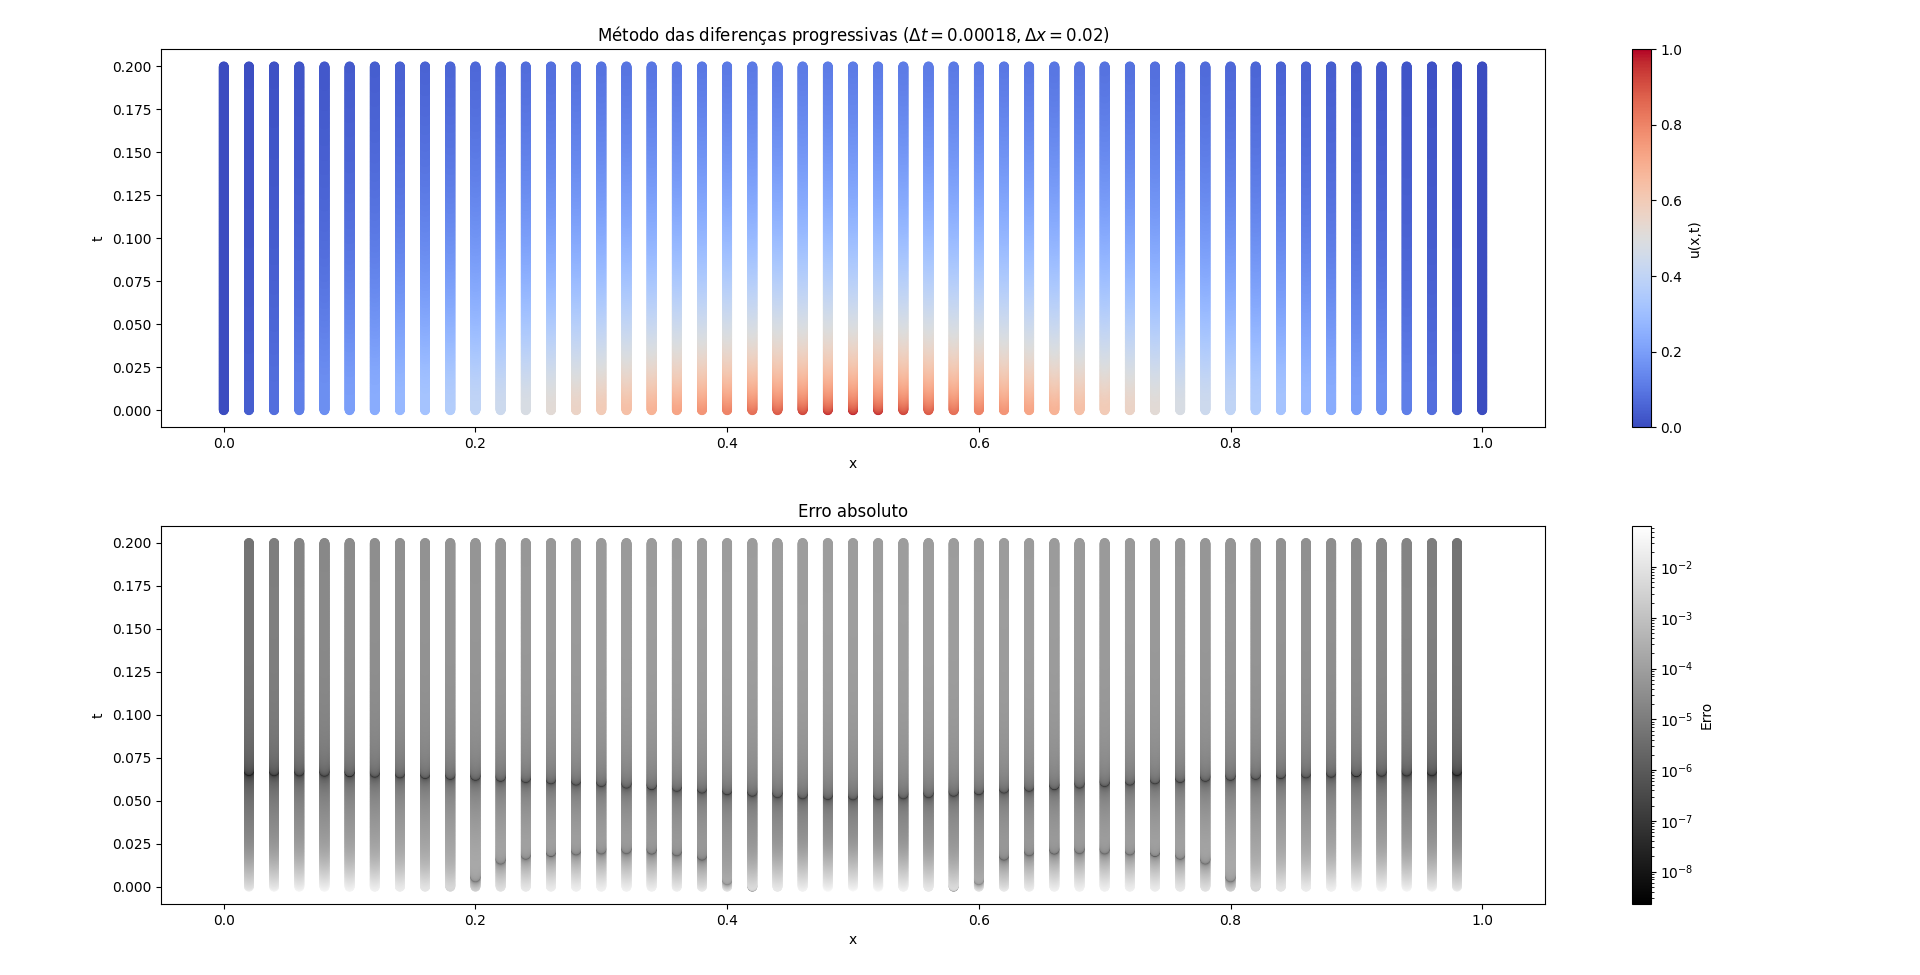
\includegraphics[width=0.7\textwidth]{img/ftcs_002.png}
\end{figure}

\clearpage
\begin{figure}[ht!]
	\centering
	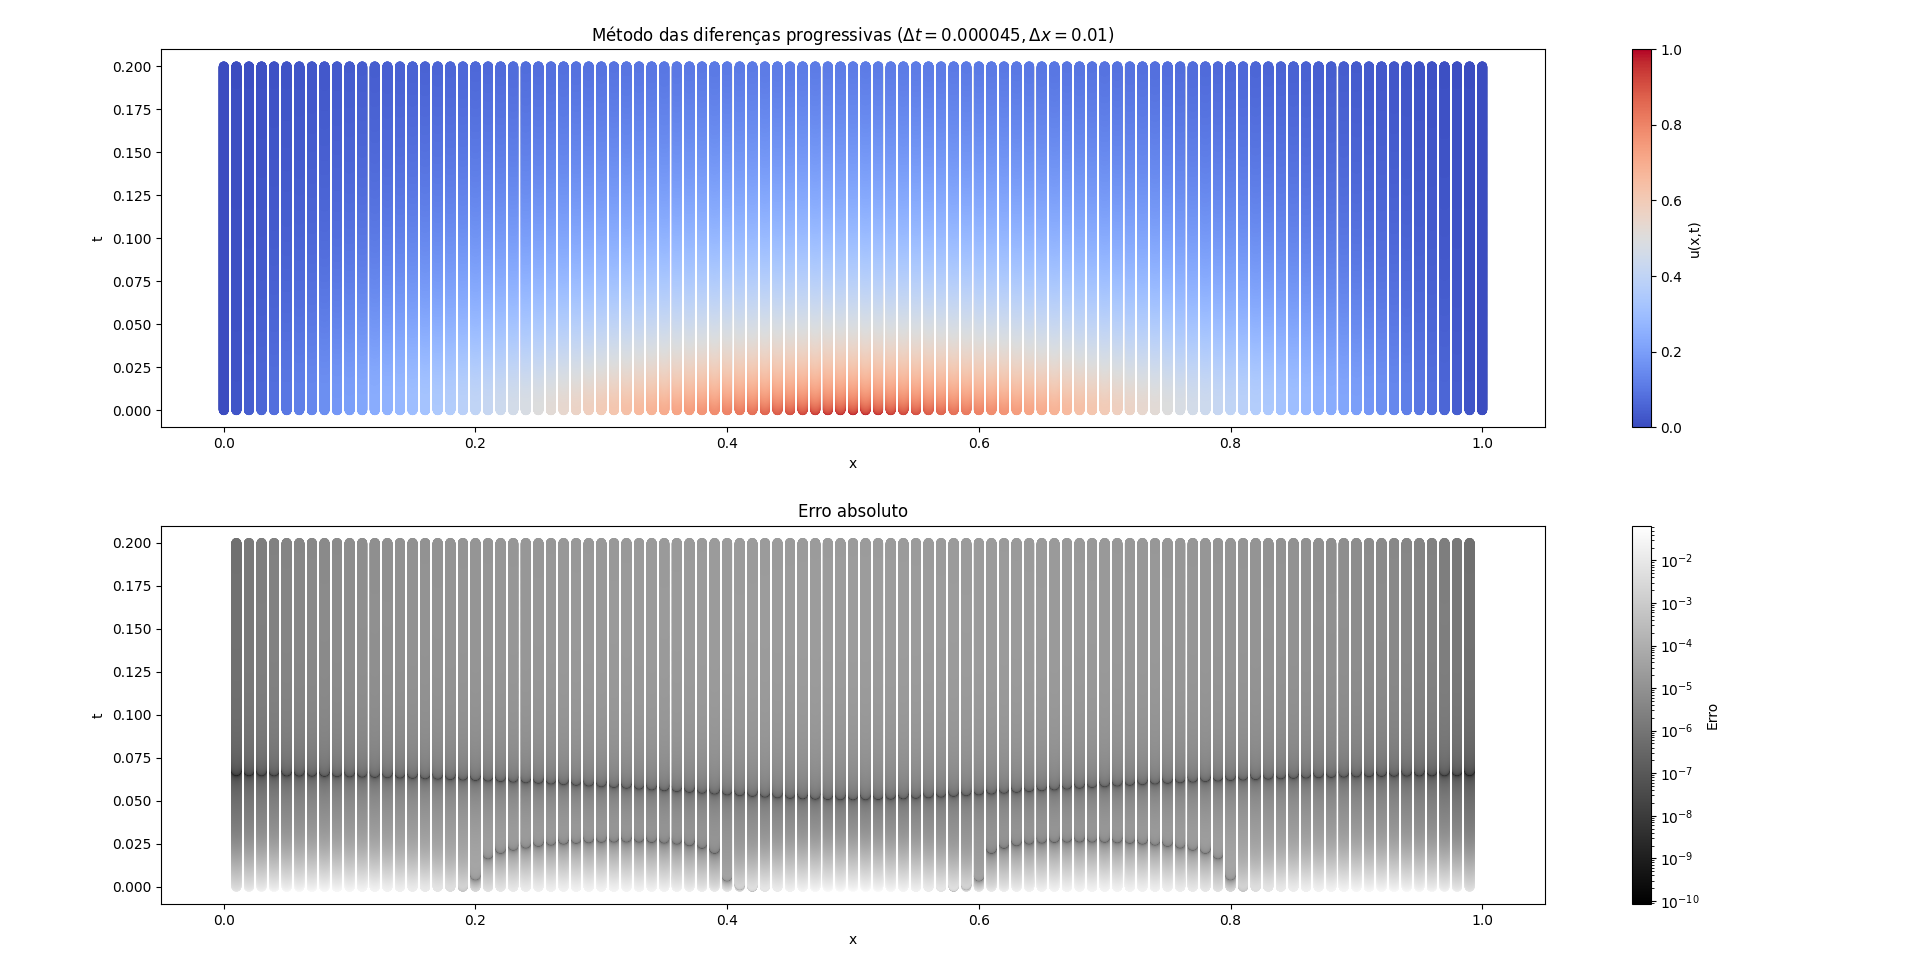
\includegraphics[width=0.7\textwidth]{img/ftcs_001.png}
\end{figure}

Nota-se, em particular, que a solução chega a um estado próximo do estacionário muito rápido, visto que os mapas de calor mostram $t$ no intervalo $[0, 0.02]$. O erro absoluto é calculado como $u(x_m, t_j) - u_{m, j}$, onde $u(x, t)$ é a aproximação pela série de Fourier do item (2.1) e $u_{m, j}$ é a aproximação gerada pelo método.

\separator

\vs
2.3. O método de diferenças progressivas foi utilizado no item (2.2), com a proporção $\mu = \frac{5}{11}$. Como comentado anteriormente, com $\mu = \frac{5}{9} > \frac{1}{2}$, os valores gerados pelo método explodiram rapidamente e não foi possível gerar um gráfico. Sabe-se que o mesmo não ocorre com o método de diferenças regressivas e o método de Crank-Nicolson:
\begin{flalign}
	u_{m, j + 1} &= u_{m, j} + \mu (u_{m - 1, j + 1} - 2 u_{m, j + 1} + u_{m + 1, j + 1}); \nonumber \\
	u_{m, j + 1} &= u_{m, j} + \frac{\mu}{2} (u_{m - 1, j} - 2 u_{m, j} + u_{m + 1, j} + u_{m - 1, j + 1} - 2 u_{m, j + 1} + u_{m + 1, j + 1}). \nonumber
\end{flalign}
Por serem métodos implícitos, a implementação desses métodos envolve resolver um sistema linear a cada passo $j$:
\begin{lstlisting}
void btcs(double x_0, double X, double t_0, double T, double dx, double dt){
	const int M = (X - x_0) / dx;
	const int N = (T - t_0) / dt;
	const double mu {dt / (dx * dx)};

	std::vector<double> x(M + 1);
	std::vector<double> t(N + 1);
	std::vector<std::vector<double>> u(N + 1, std::vector<double>(M + 1));

	for (int m {}; m <= M; m++)
	x[m] = x_0 + m * dx;

	for (int j {}; j <= N; j++)
	t[j] = t_0 + j * dt;

	for (int m {}; m <= M; m++)
	u[0][m] = f(x_0 + m * dx);

	for (int j {}; j <= N; j++){
		u[j][0] = 0;
		u[j][M] = 0;
	}

	std::vector<double> a(M - 1, -mu);
	std::vector<double> b(M - 1, 1 + 2 * mu);
	std::vector<double> c(M - 1, -mu);

	for (int j {}; j < N; j++){
		a[0] = 0;
		c[M - 2] = 0;

		std::vector<double> d(M - 1);
		for (int m {1}; m < M; m++)
		d[m - 1] = u[j][m];

		std::vector<double> solution = solveTridiagonal(a, b, c, d);
		for (int m {1}; m < M; m++)
		u[j + 1][m] = solution[m - 1];
	}
}

void crankNicolson(double x_0, double X, double t_0, double T, double dx, double dt){
	const int M = (X - x_0) / dx;
	const int N = (T - t_0) / dt;
	const double mu {dt / (dx * dx)};

	std::vector<double> x(M + 1);
	std::vector<double> t(N + 1);
	std::vector<std::vector<double>> u(N + 1, std::vector<double>(M + 1));

	for (int m {}; m <= M; m++)
	x[m] = x_0 + m * dx;

	for (int j {}; j <= N; j++)
	t[j] = t_0 + j * dt;

	for (int m {}; m <= M; m++)
	u[0][m] = f(x_0 + m * dx);

	for (int j {}; j <= N; j++){
		u[j][0] = 0;
		u[j][M] = 0;
	}

	std::vector<double> a(M - 1, -mu);
	std::vector<double> b(M - 1, 1 + 2 * mu);
	std::vector<double> c(M - 1, -mu);

	for (int j {}; j < N; j++){
		a[0] = 0;
		c[M - 2] = 0;

		std::vector<double> d(M - 1);
		for (int m {1}; m < M; m++)
		d[m - 1] = u[j][m];

		std::vector<double> solution = solveTridiagonal(a, b, c, d);
		for (int m {1}; m < M; m++)
		u[j + 1][m] = solution[m - 1];
	}
}
\end{lstlisting}

As implementações são extremamente parecidas, utilizando a mesma resolução do sistema linear por meio de uma eliminação gaussiana específica para a matriz tridiagonal destes métodos. Assim como para o método de diferenças progressivas no item (2.2), foram testados os valores $\mu = \frac{5}{9}$ e $\mu = \frac{5}{11}$. Aqui, no entanto, é importante pontuar que os métodos são incondicionalmente estáveis, então não há nenhum problema de convergência.

\separator

\vs
2.4. Como mencionado no item (2.2), todos os gráficos já ilustram o erro $u(x_m, t_j) - u_{m, j}$, onde $u(x, t)$ é a série de Fourier, considerada aqui como a solução exata.

\begin{figure}[ht!]
	\centering
	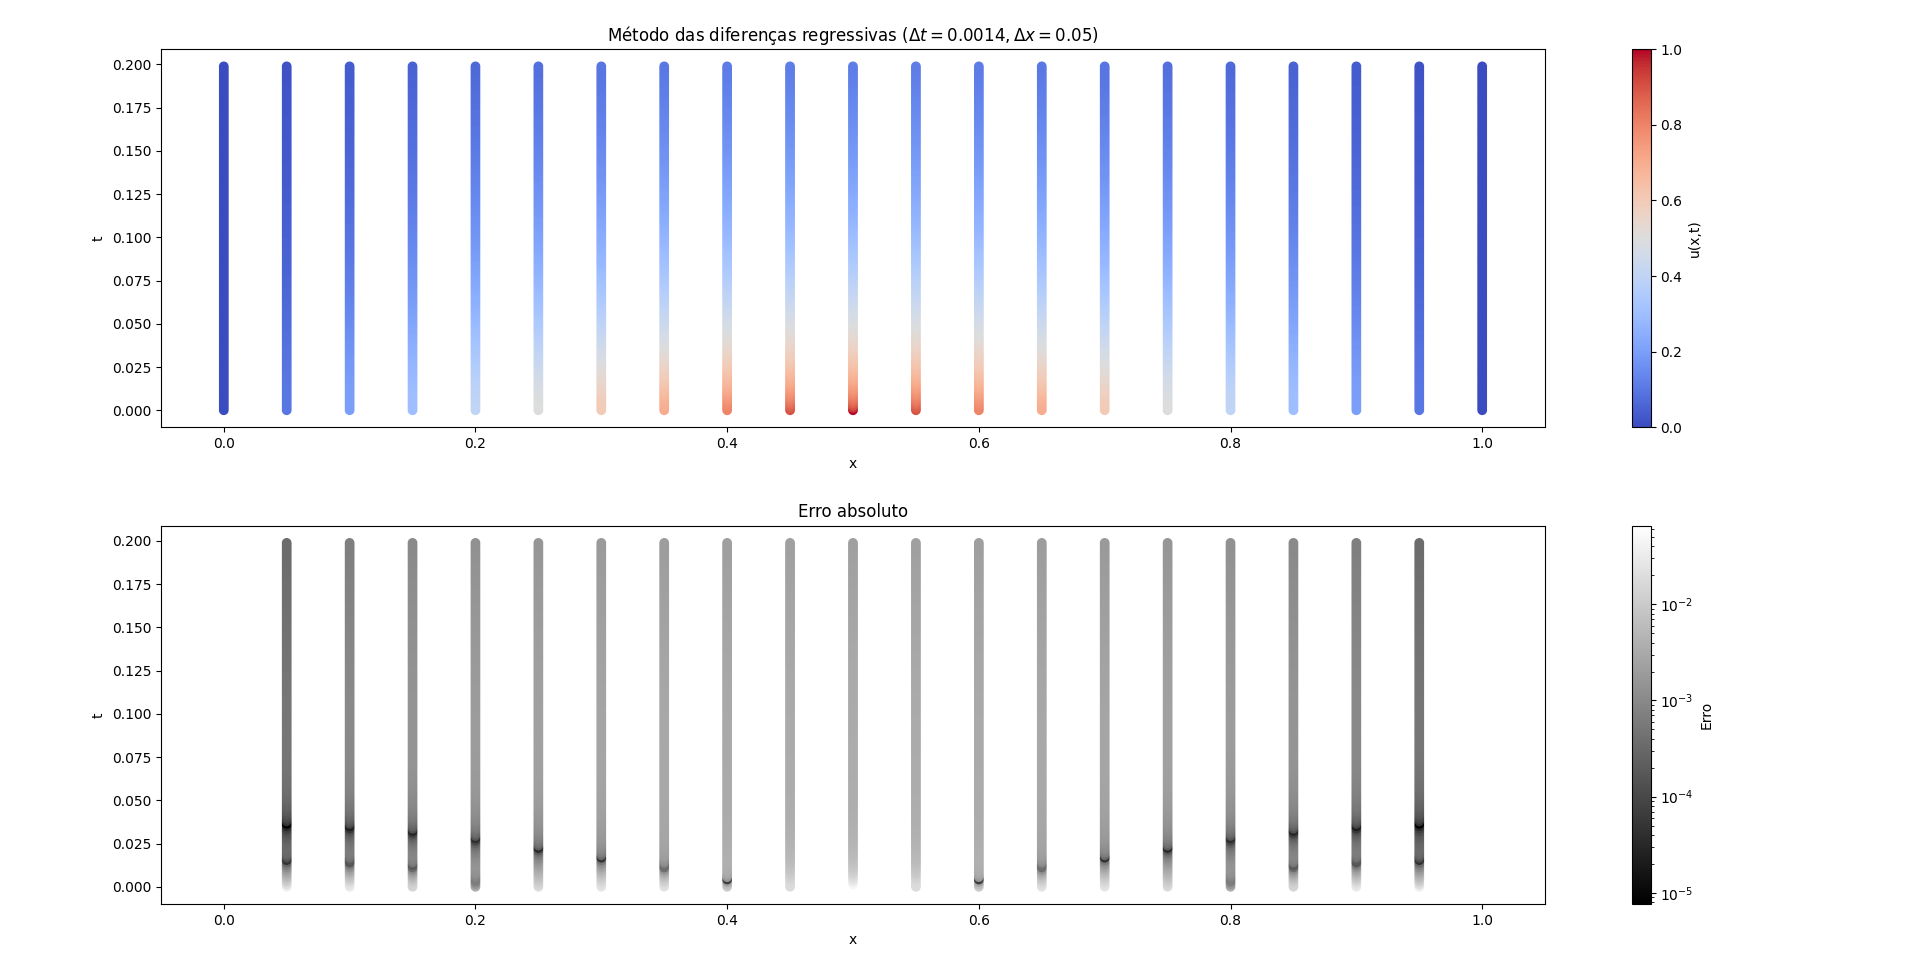
\includegraphics[width=0.7\textwidth]{img/btcs_005_9.png}
\end{figure}

\begin{figure}[ht!]
	\centering
	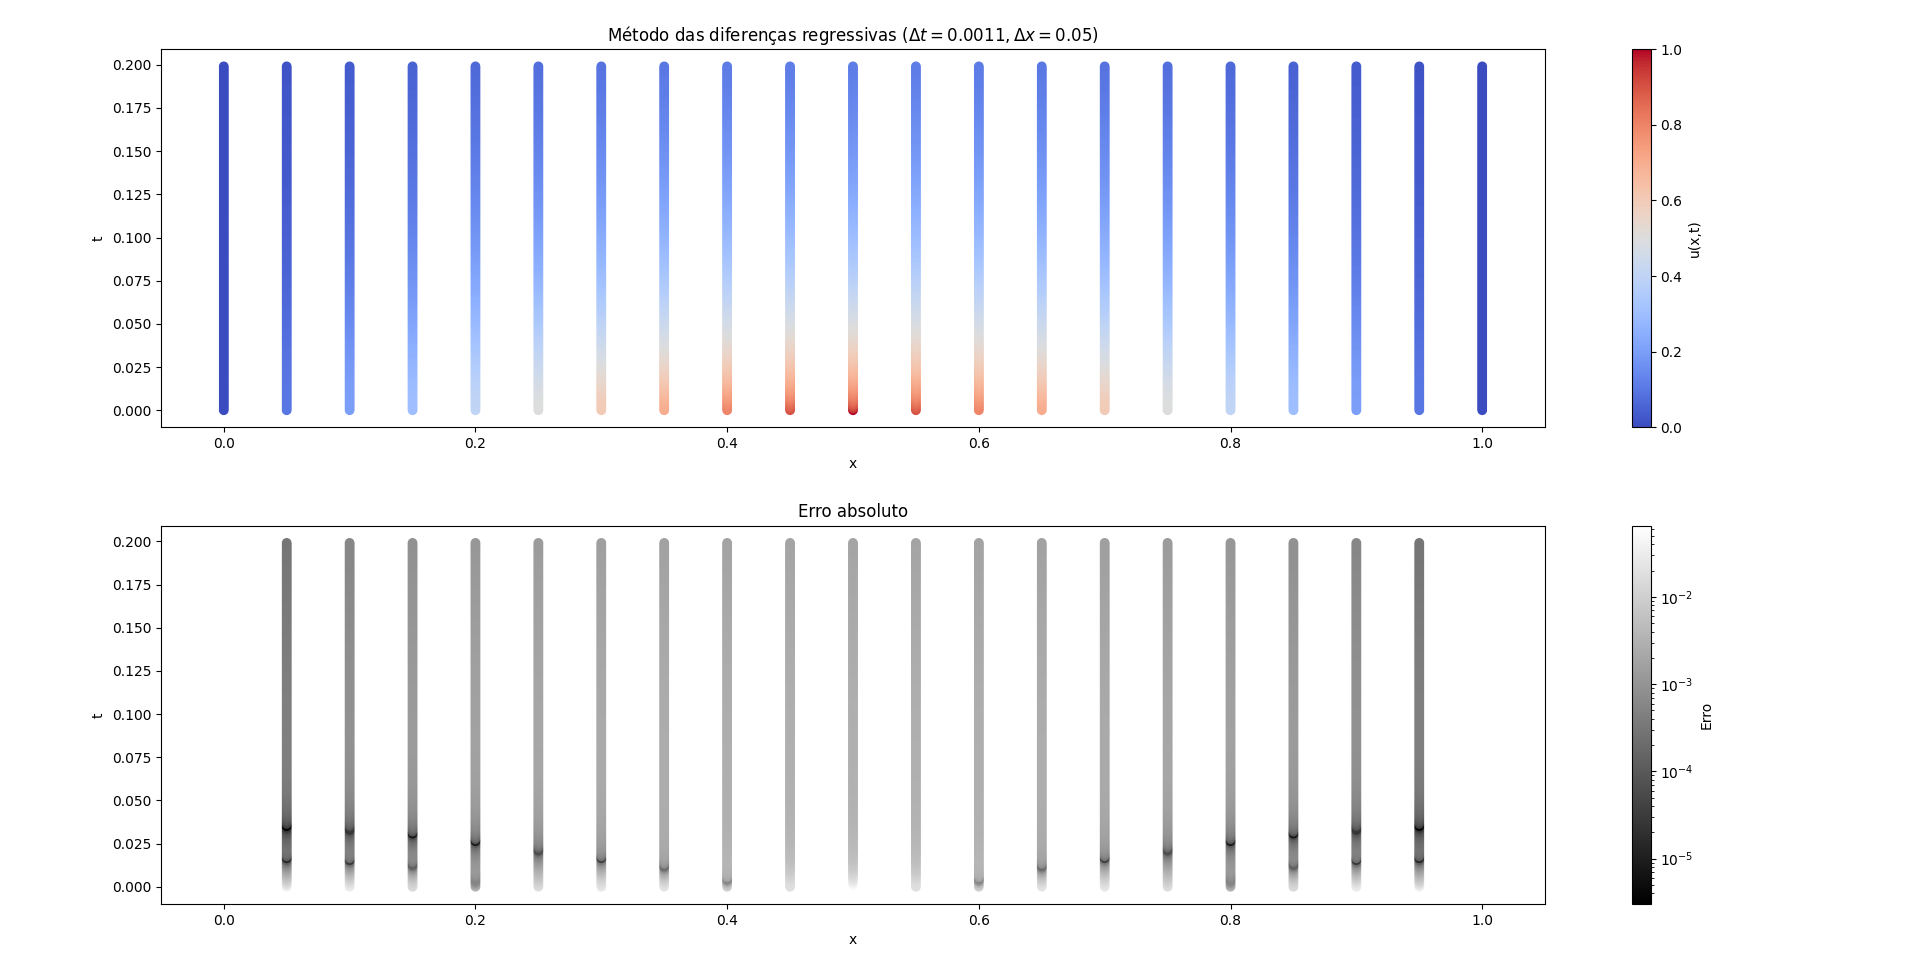
\includegraphics[width=0.7\textwidth]{img/btcs_005_11.png}
\end{figure}

\begin{figure}[ht!]
	\centering
	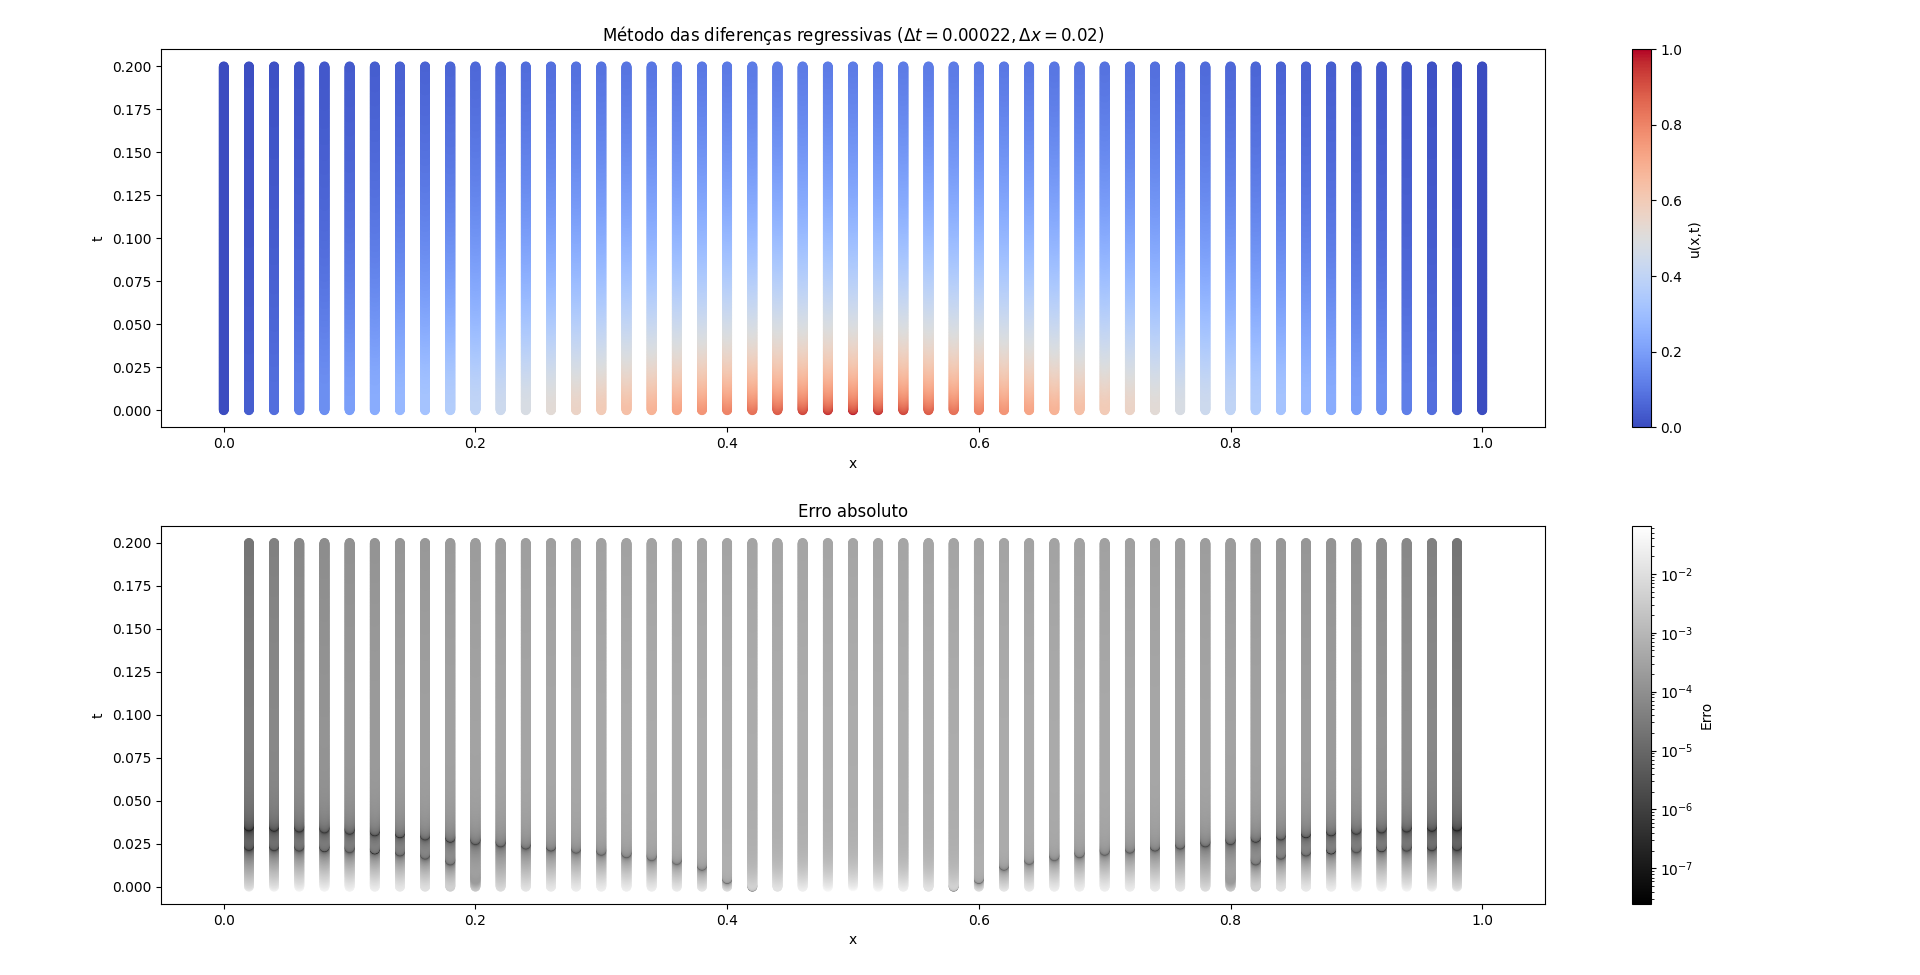
\includegraphics[width=0.7\textwidth]{img/btcs_002_9.png}
\end{figure}

\begin{figure}[ht!]
	\centering
	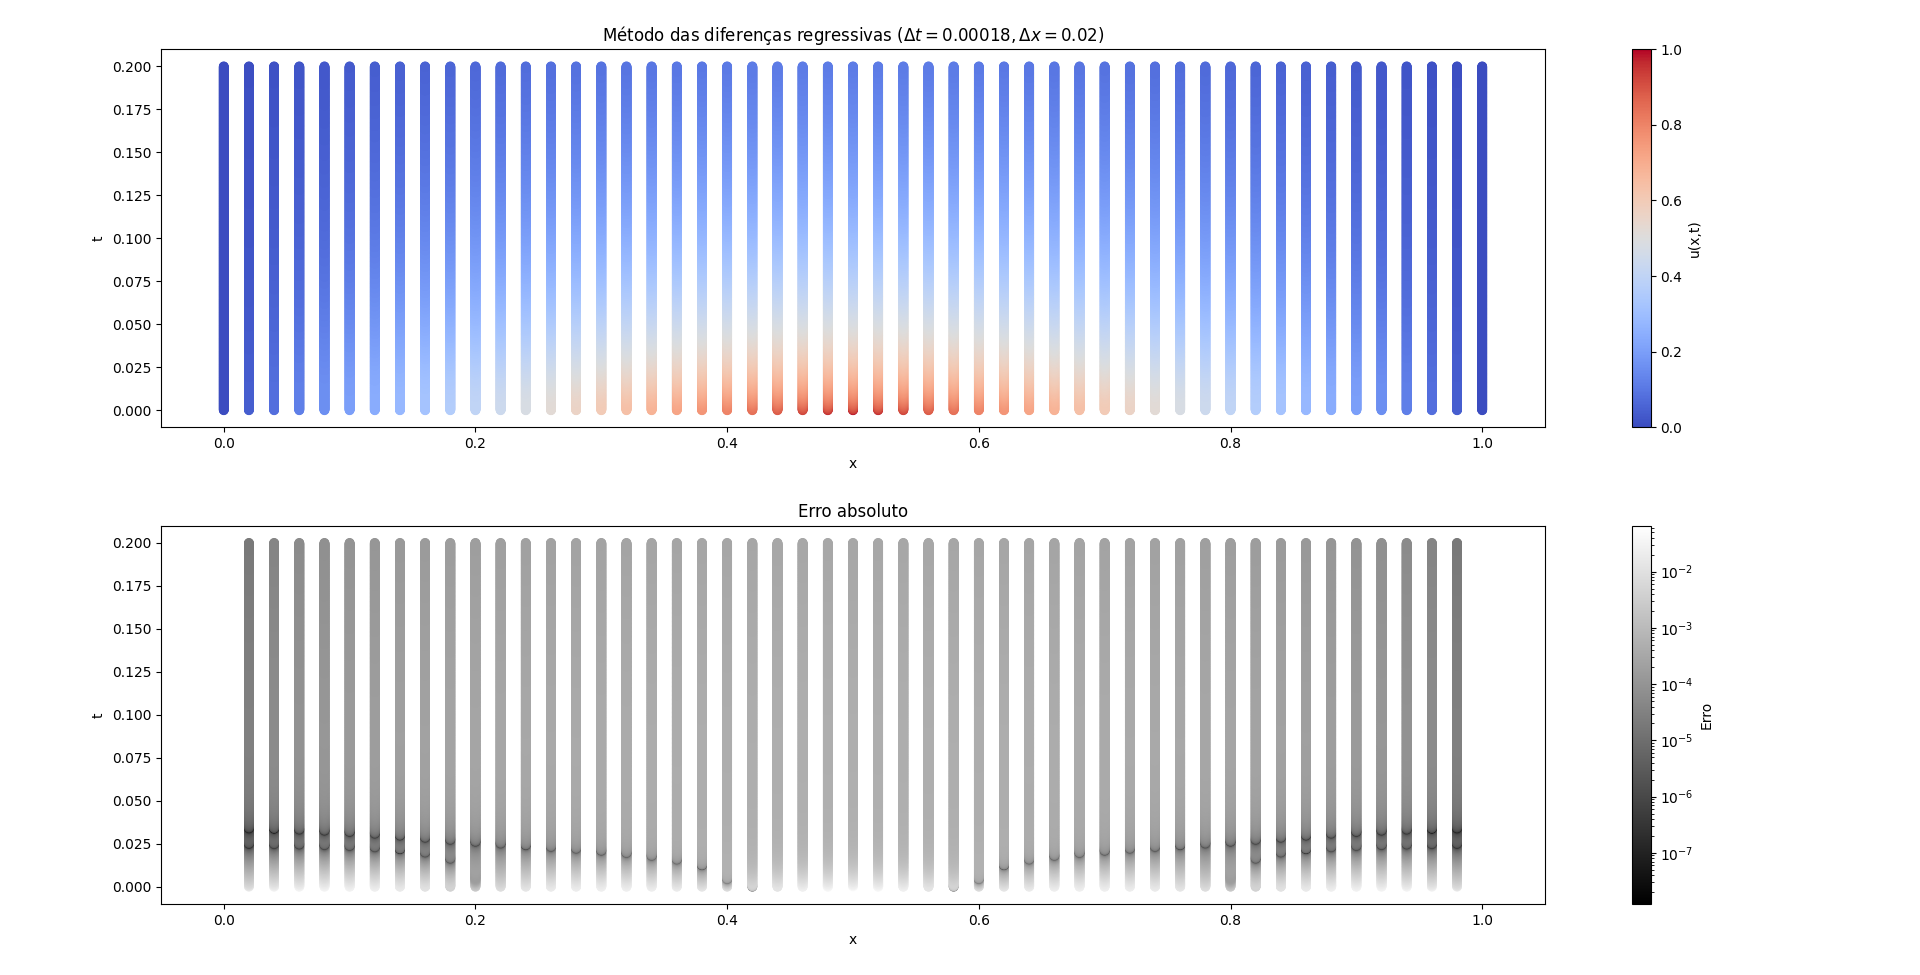
\includegraphics[width=0.7\textwidth]{img/btcs_002_11.png}
\end{figure}



\end{document}
